\subsection{Membuat project baru}
Berikut ini adalah langkah-langkah yang digunakan untuk membuat New Project
pada Quartus Prime Lite.

\framebox[1.1\width]{\textbf{Langkah 1}}
Pilih menu: \textbf{File $\rightarrow$ New Project Wizard}.
Jendela baru seperti pada gambar berikut akan
muncul.
Centang \textbf{Don't show me this introduction again} jika perlu.
Klik \textbf{Next}.
\begin{figure}[H]
\centering
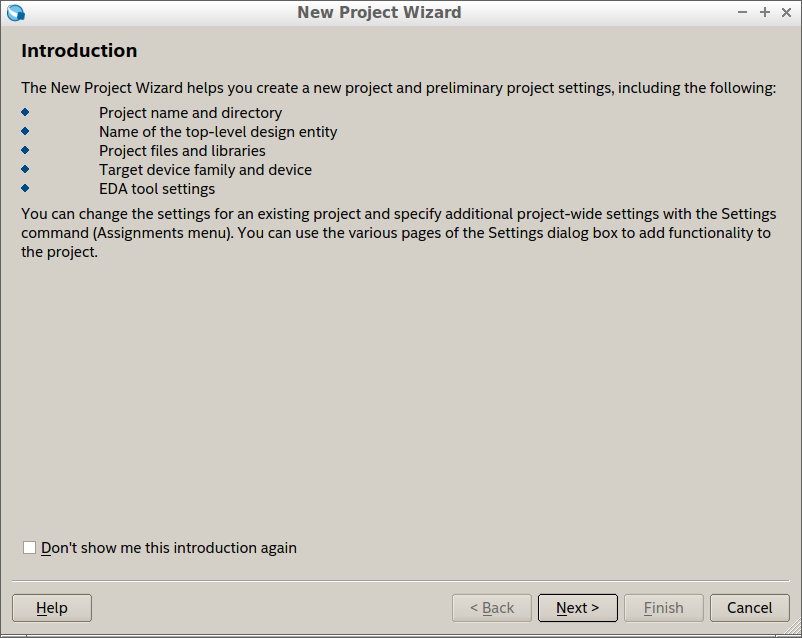
\includegraphics[width=0.5\textwidth]{images/NewProjectWizard_1.png}
\par
\end{figure}


\framebox[1.1\width]{\textbf{Langkah 2}}
Tentukan nama Project yang akan dibuat dan direktori di
mana file-file yang terkait dengan Project ini akan disimpan. Contoh
dapat dilihat pada gambar berikut. Setelah itu, klik \textbf{Next}
setelah semua isian diberikan.

\begin{figure}[H]
\centering
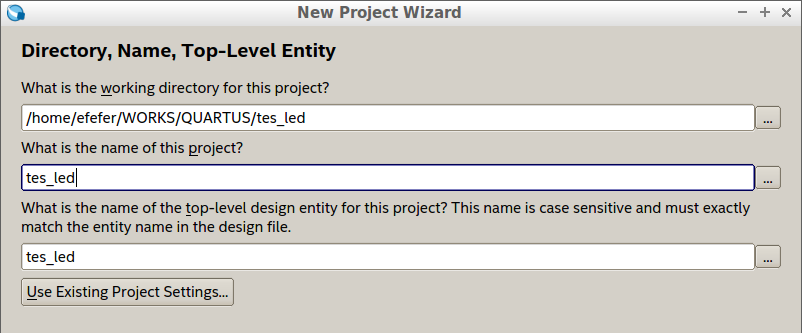
\includegraphics[width=0.5\textwidth]{images/NewProjectWizard_2.png}
\par
\end{figure}


\framebox[1.1\width]{\textbf{Langkah 3}}
Kita diminta untuk memilih jenis Project. Pilih \textbf{Empty Project}.
Setelah itu, klik \textbf{Next}.

\begin{figure}[H]
\centering
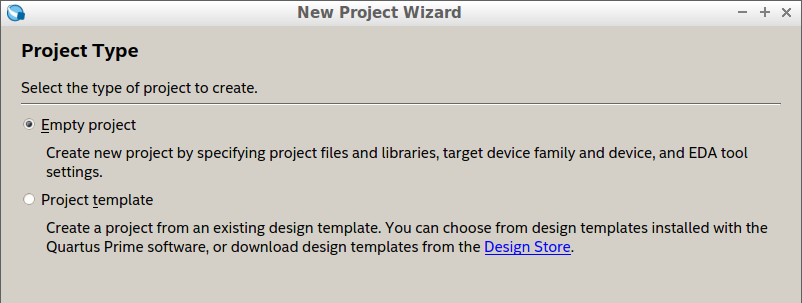
\includegraphics[width=0.5\textwidth]{images/NewProjectWizard_3.png}
\par
\end{figure}


\framebox[1.1\width]{\textbf{Langkah 4}}
Pada langkah ini kita dapat menambahkan file yang sudah ada ke Project
yang akan dibuat. Jika tidak ada langkah ini dapat dilewati.
Klik \textbf{Next}.

\begin{figure}[H]
\centering
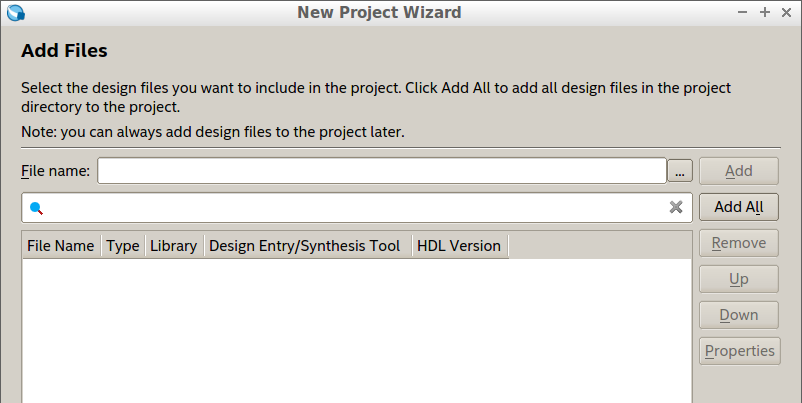
\includegraphics[width=0.5\textwidth]{images/NewProjectWizard_4.png}
\par
\end{figure}

\framebox[1.1\width]{\textbf{Langkah 5}}
Pada langkah ini, kita harus memilih \textbf{Device Family} dan
\textbf{Name}. Untuk \textbf{Device Family} pilih \textbf{Cyclone IV E}.

\begin{figure}[H]
\centering
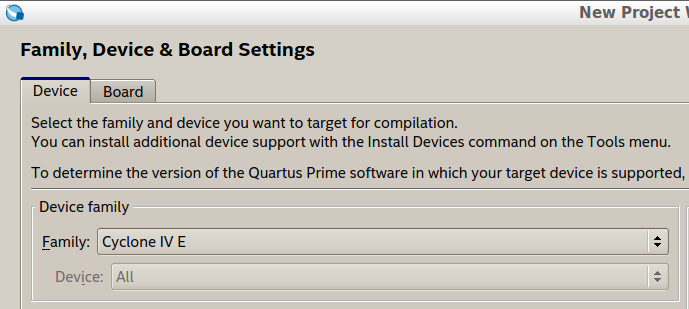
\includegraphics[width=0.5\textwidth]{images/NewProjectWizard_5_device_family.png}
\par
\end{figure}

Pada \textbf{Available Device} pilih \textbf{EP4CE6E22C8}.
Setelah itu, klik \textbf{Next}.

\begin{figure}[H]
\centering
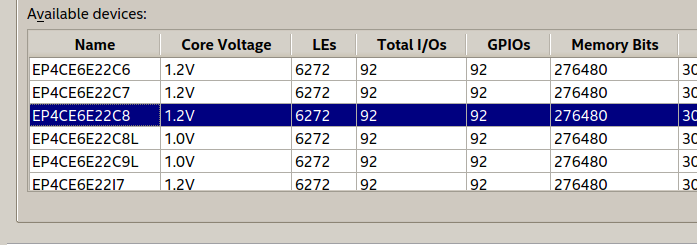
\includegraphics[width=0.5\textwidth]{images/NewProjectWizard_5_device_name.png}
\par
\end{figure}


\framebox[1.1\width]{\textbf{Langkah 6}}
Quartus akan meminta kita untuk memilih setting beberapa tools yang
mungkin digunakan. Untuk sementara pilih \textbf{None} untuk semua tools.
Setelah itu, klik \textbf{Next}.

\begin{figure}[H]
\centering
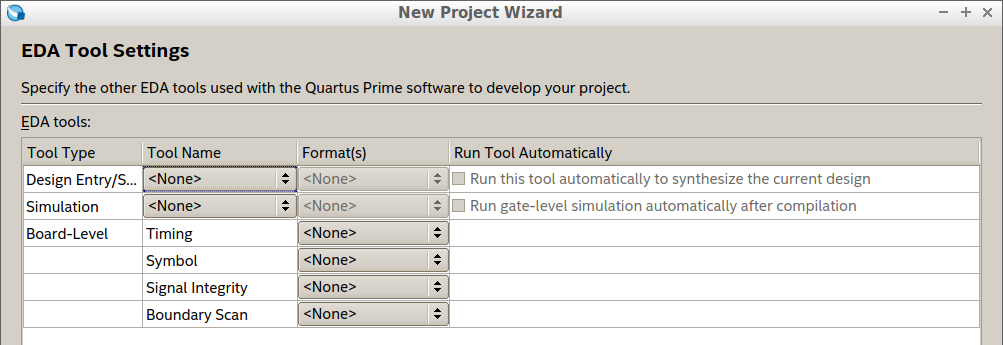
\includegraphics[width=0.5\textwidth]{images/NewProjectWizard_6.png}
\par
\end{figure}

\framebox[1.1\width]{\textbf{Langkah 7}}
Pada bagian akhir, Quartus akan memberikan Summary dari Project yang akan
dibuat. Setelah itu, klik \textbf{Finish}.
\begin{figure}[H]
\centering
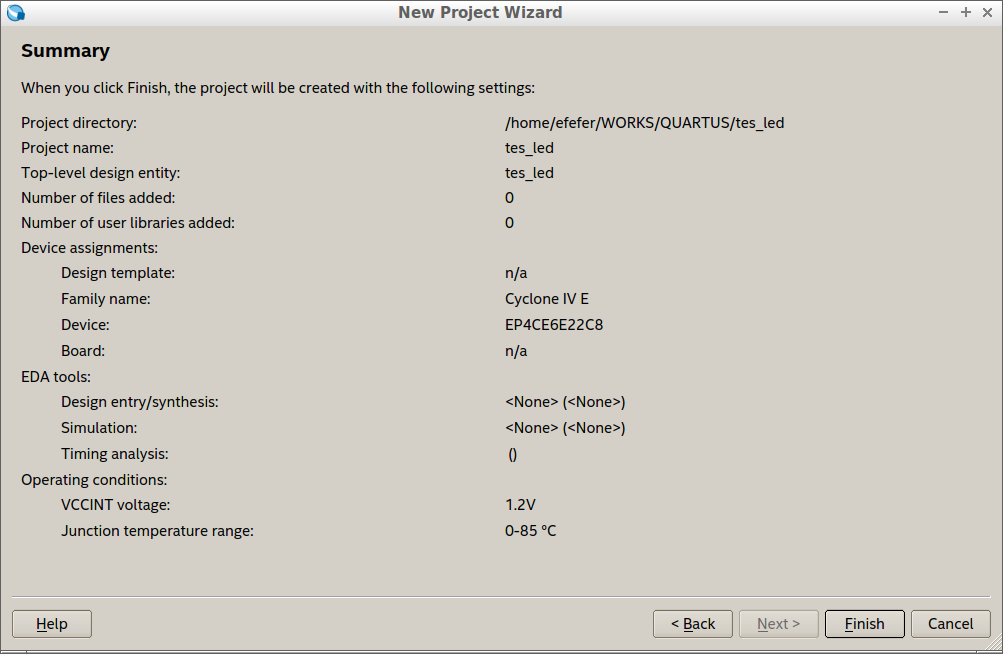
\includegraphics[width=0.5\textwidth]{images/NewProjectWizard_7.png}
\par
\end{figure}


